\section{Evidence for the SM Higgs} \label{sec:higgs:higgs_evidence}

Using the above information about predicted final states the CMS and ATLAS
experiment collaborations analyszed 5 $\text{fb}^{-1}$ of LHC Run 1 data 
\cite{Khachatryan:2016vau} to make measurements of the SM Higgs production 
cross-sections and branching ratios.  The combined results of these studies 
can be seen in \Cref{fig:higgs_production_measurement} 
\Cref{fig:higgs_decay_measurement_1} and \Cref{fig:higgs_decay_measurement_2}.  
Given the uncertanties on the measurements these results show good agreement 
between the predictions of the Standard Model and experiment with all best 
fit values falling within $2\sigma$ of the SM theoretical prediction.

\begin{figure}[!htbp]
  \begin{center}
    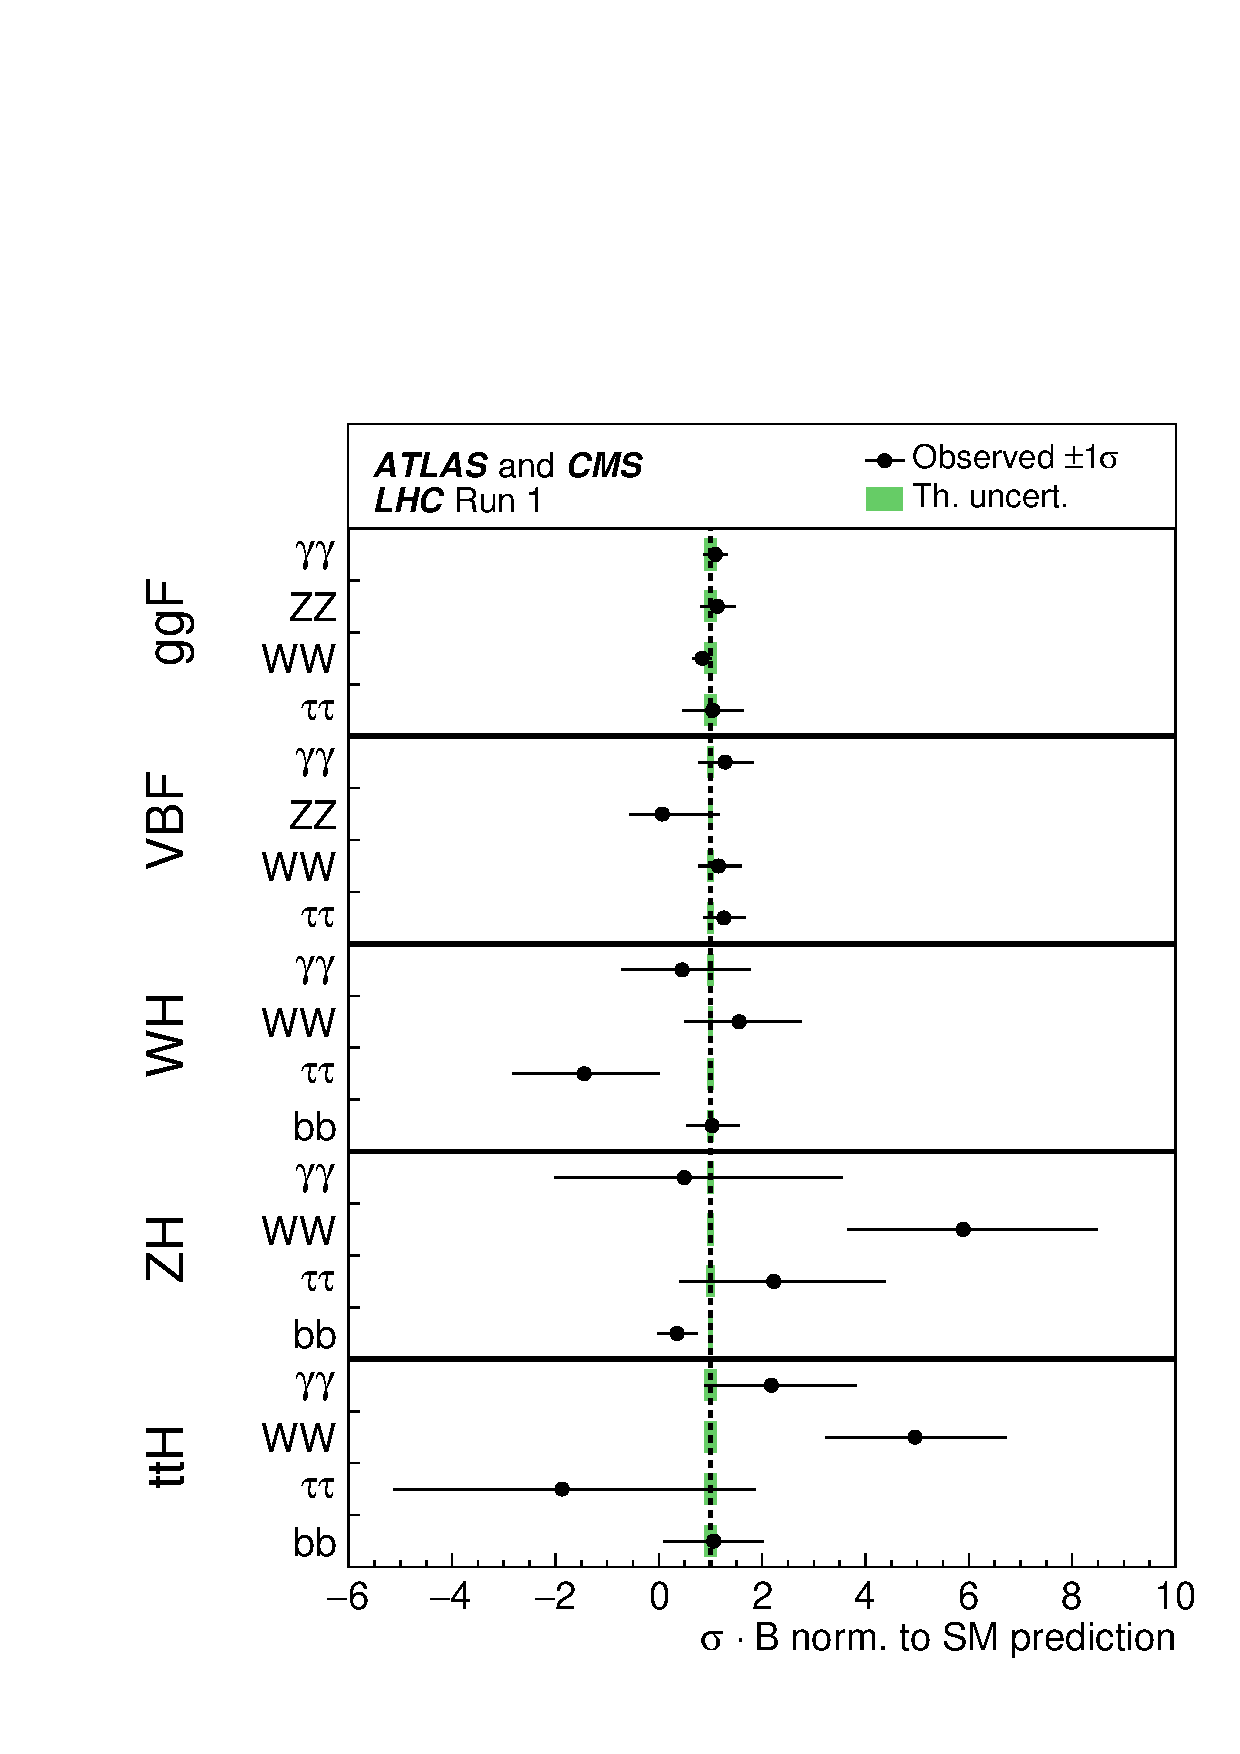
\includegraphics[width=0.5\linewidth]{figures/higgs/higgs_production_measurement.pdf}
    \caption{ Best fit values of $\sigma_{i} \cdot B^{f}$ for each specific channel $i \rightarrow H \rightarrow f$, as obtained from the generic parameterisation with 23 parameters for the combination of the ATLAS and CMS measurements. The error bars indicate the $1\sigma$ intervals. The fit results are normalised to the SM predictions for the various parameters and the shaded bands indicate the theoretical uncertainties in these predictions. Only 20 parameters are shown because some are either not measured with a meaningful precision, in the case of the $H \rightarrow ZZ$ decay channel for the $WH$, $ZH$, and $t\bar{t}H$ production processes, or not measured at all and therefore fixed to their corresponding SM predictions, in the case of the H → bb decay mode for the ggF and VBF production processes \cite{Khachatryan:2016vau}.}
    \label{fig:higgs_production_measurement}
  \end{center}
\end{figure}

\begin{figure}[!htbp]
  \begin{center}
    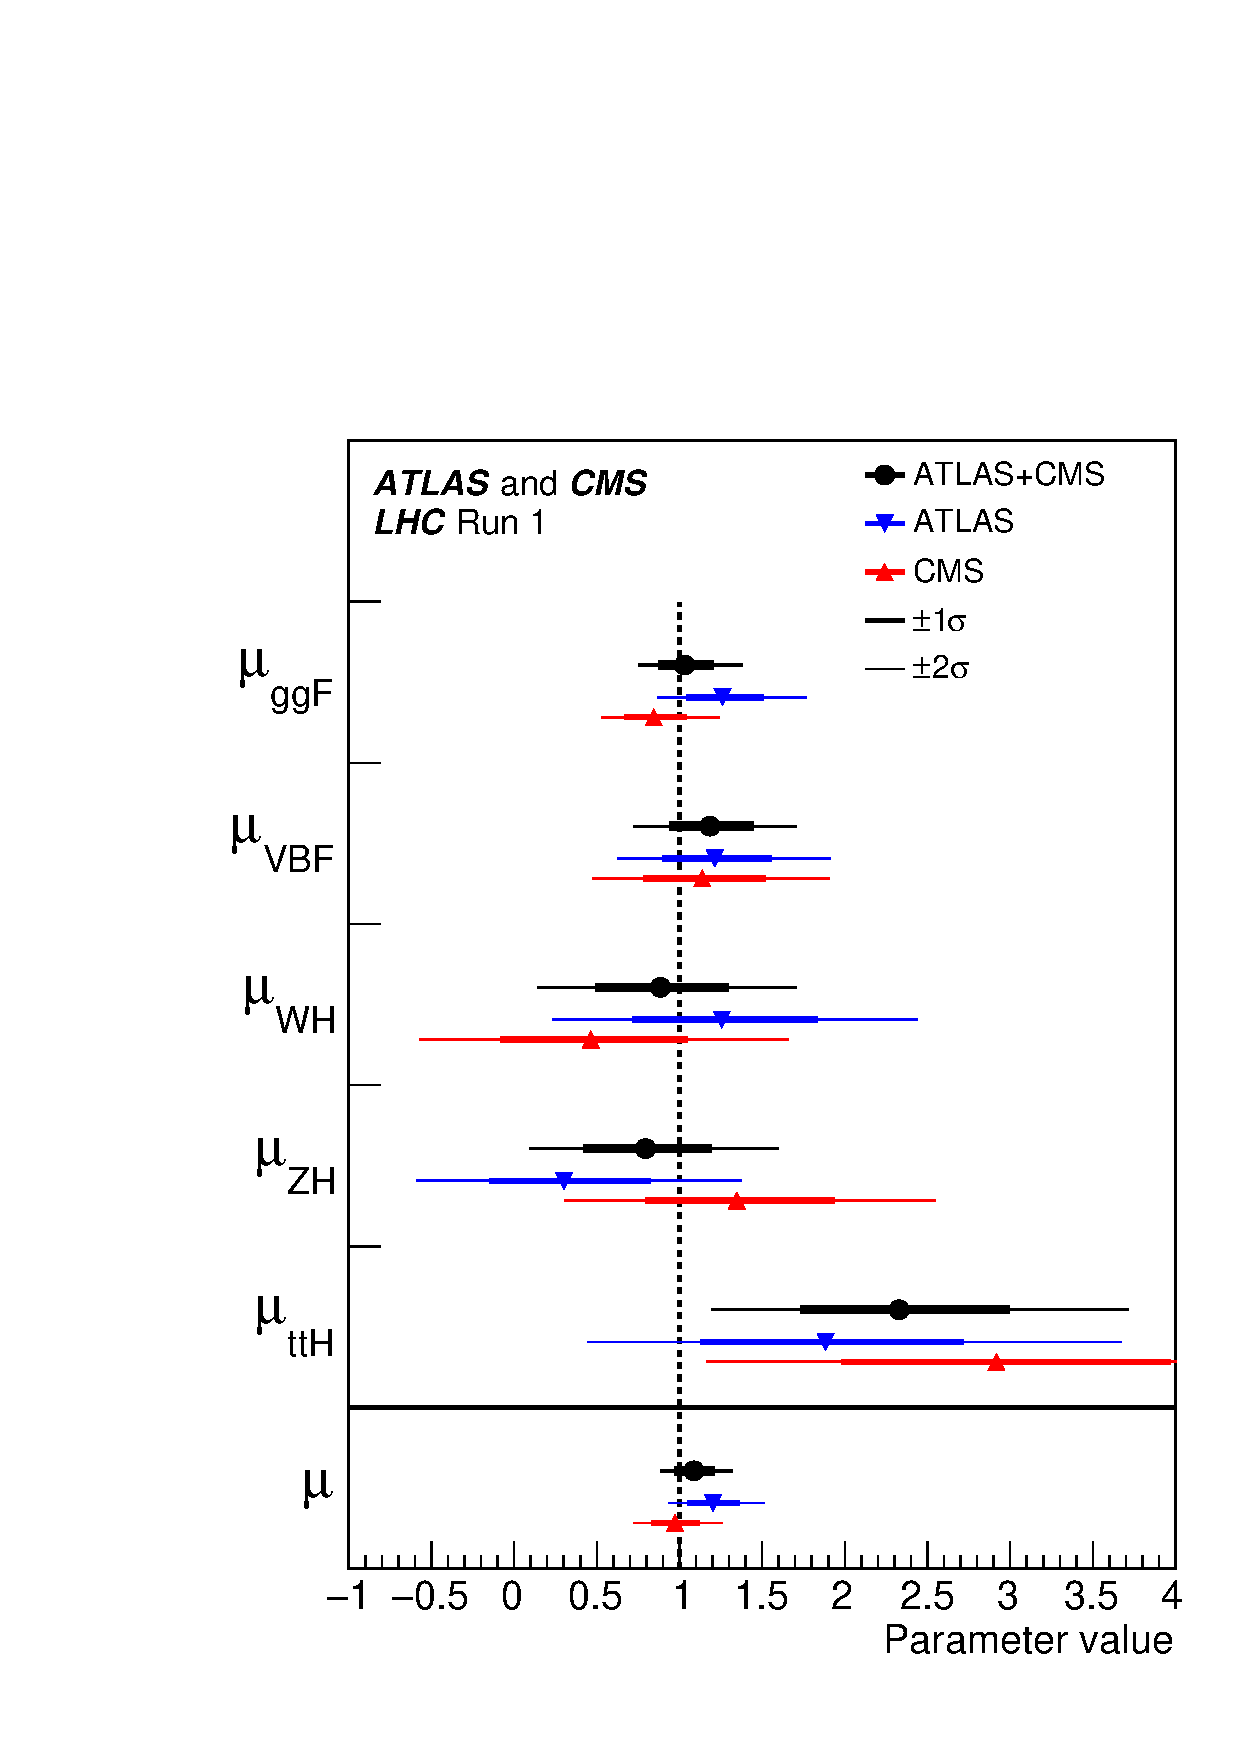
\includegraphics[width=0.5\linewidth]{figures/higgs/higgs_decay_measurement_1.pdf}
    \caption{Best fit results for the production signal strengths for the combination of ATLAS and CMS data. Also shown are the results from each experiment. The error bars indicate the $1\sigma$ (thick lines) and $2\sigma$ (thin lines) intervals. The measurements of the global signal strength $\mu$ are also shown \cite{Khachatryan:2016vau}.}
    \label{fig:higgs_decay_measurement_1}
  \end{center}
\end{figure}

\begin{figure}[!htbp]
  \begin{center}
    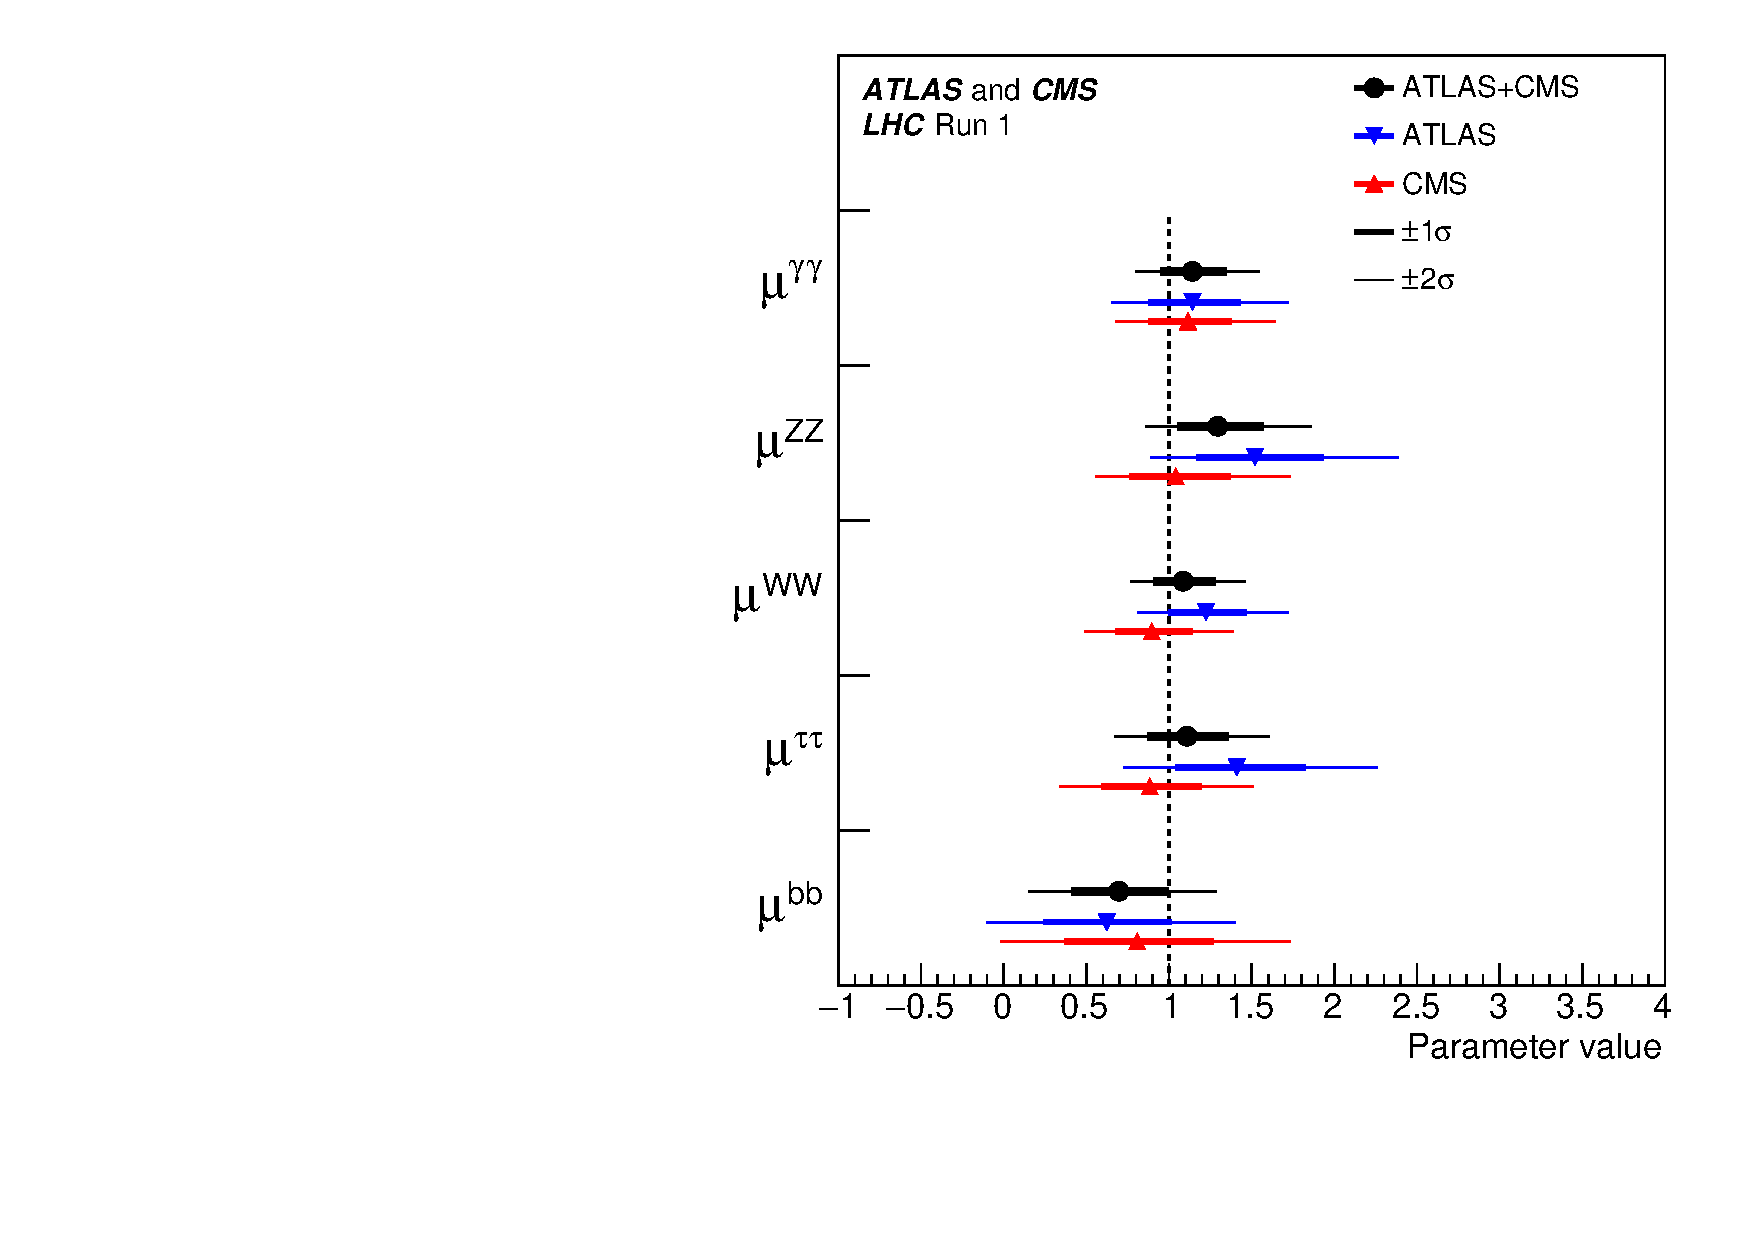
\includegraphics[width=0.5\linewidth]{figures/higgs/higgs_decay_measurement_2.pdf}
    \caption{ Best fit results for the decay signal strengths for the combination of ATLAS and CMS data. Also shown are the results from each experiment. The error bars indicate the $1\sigma$ (thick lines) and $2\sigma$ (thin lines) intervals \cite{Khachatryan:2016vau}.}
    \label{fig:higgs_decay_measurement_2}
  \end{center}
\end{figure}
